\documentclass{beamer}
\usepackage{ctex}
\usepackage{graphicx}
\usepackage{amsmath}
\usepackage{booktabs}
\usepackage{hyperref}
\usepackage{subcaption}
\usepackage{multicol}
\usepackage{listings}
\usepackage{multirow}
\usepackage{tabularx}

\bibliographystyle{alpha}

\usetheme{Madrid}
\usecolortheme{seahorse}

% 自定义块颜色
\setbeamercolor{block title}{bg=blue!30,fg=black}
\setbeamercolor{block body}{bg=blue!10,fg=black}
\setbeamercolor{exampleblock title}{bg=green!50,fg=black}
\setbeamercolor{exampleblock body}{bg=green!20,fg=black}

% 开启图表编号
\setbeamertemplate{caption}[numbered]

\title{\textbf{周报-向嘉豪(2024-11-25)}}
\author{向嘉豪}
\institute{衡阳师范学院}
\date{2024年11月25日}

\begin{document}

\begin{frame}
    \titlepage
\end{frame}

\begin{frame}
    \frametitle{摘要}
       \begin{block}{本周工作取得三项主要进展}
        \begin{enumerate}
            \item 完成LCB基准测试框架的跨平台扩展,成功将ESP32S3纳入测试平台,并通过QARMAv2算法性能评测验证框架的可扩展性。
            \item 论文撰写完成初稿,完善了算法优化方法、实验结果分析和结论展望等核心章节。经查重,相似度为9\%,符合学术规范。
            \item 基于IEEE期刊推荐系统,筛选出4个潜在目标期刊,其中\textbf{IEEE Transactions on Information Forensics and Security}(IF=6.3)因研究方向契合、影响因子高,确定为首选投稿目标。
        \end{enumerate}
    \end{block}
\end{frame}


\section{LCB框架跨平台扩展}
\begin{frame}
    \frametitle{LCB框架跨平台扩展}
    为验证LCB基准测试框架的跨平台通用性,本周成功将支持平台扩展至\textbf{ESP32S3}。通过在该平台上对\textbf{QARMAv2}加密算法进行系统性能评测,发现相同实现在ESP32S3上的执行效率较基准平台降低约\textbf{50\%},这一结果有力证实了硬件平台特性对加密算法性能的显著影响。
\end{frame}

\section{论文内容完善}
\begin{frame}
    \frametitle{论文内容完善}
    本周重点完善了论文的三个关键章节:
    \begin{itemize}
        \item 第4.1节详细阐述了\textbf{AES算法的优化实现方法}。
        \item 第4.3节系统呈现了实验环境配置、性能测试结果及其对比分析。
        \item 第5章总结了研究成果并提出未来优化方向。
    \end{itemize}
    
    论文初稿已完成,并经查重系统检测,相似度为\textbf{9\%},表明内容具有良好的原创性(如图\ref{fig:check}所示)。

    \begin{figure}
        \centering
        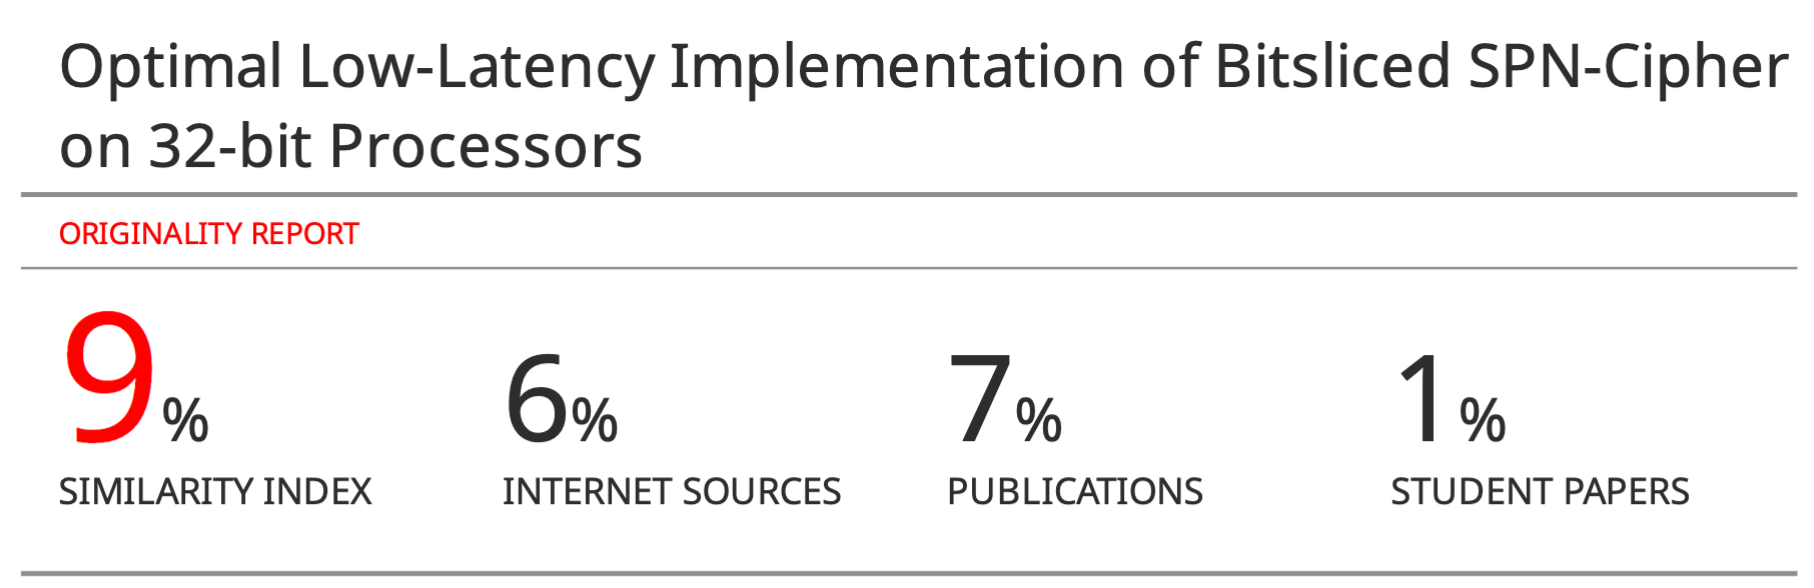
\includegraphics[width=0.8\textwidth]{./fig/duplicate_9.png}
        \caption{论文查重结果}
        \label{fig:check}
    \end{figure}
\end{frame}

\section{目标期刊甄选}
\begin{frame}
    \frametitle{目标期刊甄选}
    基于\textbf{IEEE期刊推荐系统}(\url{https://publication-recommender.ieee.org}),通过输入研究摘要获取了20个相关Trans期刊。经过对影响因子、审稿周期、期刊定位等多维度分析,筛选出4个候选期刊(详见表\ref{tab:journal})。
\end{frame}

\begin{frame}
    \frametitle{期刊对比分析及首选投稿目标}
    
    \begin{table}[ht]
      \centering
      \caption{目标期刊对比分析}
      \label{tab:journal}
      \resizebox{\textwidth}{!}{
      \begin{tabular}{lcccc}
          \toprule
          期刊名称 & 分区 & IF值 & 审稿周期(月) & 年文章数 \\
          \midrule
          IEEE Trans. on Consumer Electronics & 2区 & 4.3 & 3 & 224 \\
          IEEE Trans. on Industry Applications & 2区 & 4.2 & 3 & 769 \\
          \textbf{IEEE Trans. on Info. Forensics and Security} & 1区/CCF-A & 6.3 & 5 & 799 \\
          IEEE Trans. on Computers & 2区/CCF-A & 3.6 & 6 & 144 \\
          \bottomrule
      \end{tabular}
      }
      \small
      \caption*{年文章数:为该期刊2024年发表的文章数。审稿周期:查看最新一期的文章,计算从投稿到发表的时间,三篇取平均值。}
  \end{table}
    
    
    考虑到\textbf{Information Forensics and Security}在2022年发表过相近研究主题的文章,且具备最高影响因子(6.3)和较优审稿周期(5个月),将其确定为\textbf{首选投稿目标}。
\end{frame}

\begin{frame}
  \frametitle{老师评语}

  \begin{block}{IEEE Trans. on Info. Forensics and Security这个期刊行业内高度认可,仔细按期刊要求修改好论文,可以投}
      仔细修改,准备投稿。
  \end{block}
  \begin{alertblock}{本周计划}
      \begin{itemize}
          \item 对论文进行精细化修订。
          \item 按IEEE期刊模板重构论文格式。
      \end{itemize}
  \end{alertblock}
\end{frame}

\end{document}